\subsection{Analogschalter} % (fold)
\label{sub:Analogschalter}
\begin{frame}
\frametitle{Tiefpass}
\framesubtitle{}
    \begin{columns}[c]
        \column{0.5\textwidth}
             \begin{block}{Tiefpass}
                 \begin{itemize}
                     \item Tiefpassfilter zum ... ???
                     \item $R=10k\Omega$, $C = 10\mu F$
                     \item Grenzfrequenz 
                     \begin{equation*}
                         f_G = \frac{1}{2 \pi R C} = 1.59Hz
                     \end{equation*}
                 \end{itemize}
             \end{block}
        \column{0.5\textwidth}
        \begin{figure}[H]
        \begin{center}
                \includegraphics[scale=0.4]{./img/schaltung/Tiefpass.png}
        \end{center}
        \end{figure}
        \begin{figure}[H]
        \begin{center}
                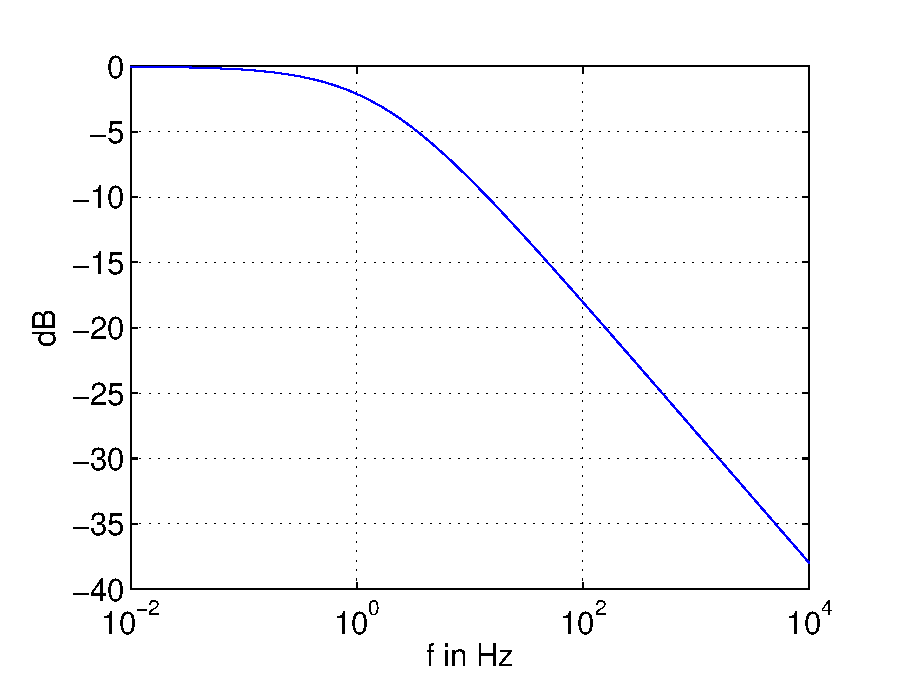
\includegraphics[scale=0.325]{./img/plots/theorie_tiefpass.eps}
        \end{center}
        \end{figure}
    \end{columns}
\end{frame}
% subsection Analogschalter (end)
